
\section{Visualization with \gnuplot}

\paragraph{Display with \gnuplot}
To display statistical information about a finished simulation run the correct \gnuplot configuration file needs to be opened with \gnuplot. On Unix systems (with installed \gnuplot) the interactive \gnuplot shell can be used ( (\texttt{> load }``\texttt{gnuplotfile.plt}''). More commands can be displayed using \texttt{> help}. Also it is possible to directly display the file with \texttt{\$ gnuplot -persist }``\texttt{gnuplotfile.plt}''. The additional option \texttt{-persist} causes the window to stay open after the file has been opened. For more informaion on \gnuplot read the manual page \texttt{\$ man gnuplot}.


\paragraph{Display configuration}
A file  \texttt{\scriptsize output\_20091224\_184129\_ALL.plt} might look like this:

\begin{center}
\texttt{\begin{tabular}{rrrl}
\# time & avg\_spd & minball\_x & (\dots) \\
\hline
0 & 9.2 & 20.5 \\
1 & 11.3 & 21.5 \\
4 & 9.1 & 21.9 \\
6 & 7.5 & 22.3
\end{tabular}}
\end{center}

Each line contains extremly valuable statistical data for a certain time. The start of a new column is marked by one (or more) whitespaces.
comment lines are started with a '\#' sign.

The file  \texttt{gnuplot\_20091224\_184129\_ALL.plt} also contains the formatting of the extremly valuable statistical data. The formatting can be changed if so desired. 

\begin{verbatim}
# statistics of the simulation
#====================================
set title ' SCHLAUE SCHWÄRME '
set xrange []
set yrange []
set grid
set pointsize 0.5
set xlabel 'time'
set ylabel ''
plot 'output_(...)_ALL.plt' using 1:2 title 'avg_spd' with linespoints,\
     'output_(...)_ALL.plt' using 1:3 title 'minball_x' with linespoints
\end{verbatim}

The lines have the following meaning:
\begin{itemize}
\item \texttt{set title '\textit{Titel}'} generates a title within the upper part of the graphical display.
\item \texttt{set xrange [\textit{min}:\textit{max}]} limits the visible area (horizontal) to the area between \texttt{\textit{min}} ans \texttt{\textit{max}}, \texttt{set xrange []} scales the extremly valuable statistical data based on the datapoints
\item \texttt{set grid} displays a beautiful grid.
\item \texttt{set pointsize \textit{multiplikator}} scales the size of the points (if there are any) according to \texttt{\textit{multiplikator}}.
\item \texttt{xlabel '\textit{Label}'} labels the x-axis with useful information.
\end{itemize}
These choices only concern the graphical display. The configuration of the displayed data is done later.

\begin{itemize}
 \item \texttt{plot '\textit{Dateiname.plt}'} starts the display process. Data is read from the input file. The parameter \texttt{using 1:2} uses the first column as x-axis and the second column as y-axis. \texttt{title `avg\_speed'} adds a title for the function defined by this. The addition \texttt{with linespoints} causes the data points to be displayed with lines between them. \texttt{linespoints} can be replaced by:
\begin{itemize}
\item \texttt{lines} connects each data point with a line
\item \texttt{dots}displays datapoints as dots (for many datapoints)
\item \texttt{points} displays datapoints as points
\item \texttt{linespoints} displays a combination of \textit{points} and \textit{lines}
\item \texttt{impulses} displays a vertical line for each data point
\end{itemize}

\end{itemize}

\begin{figure}
	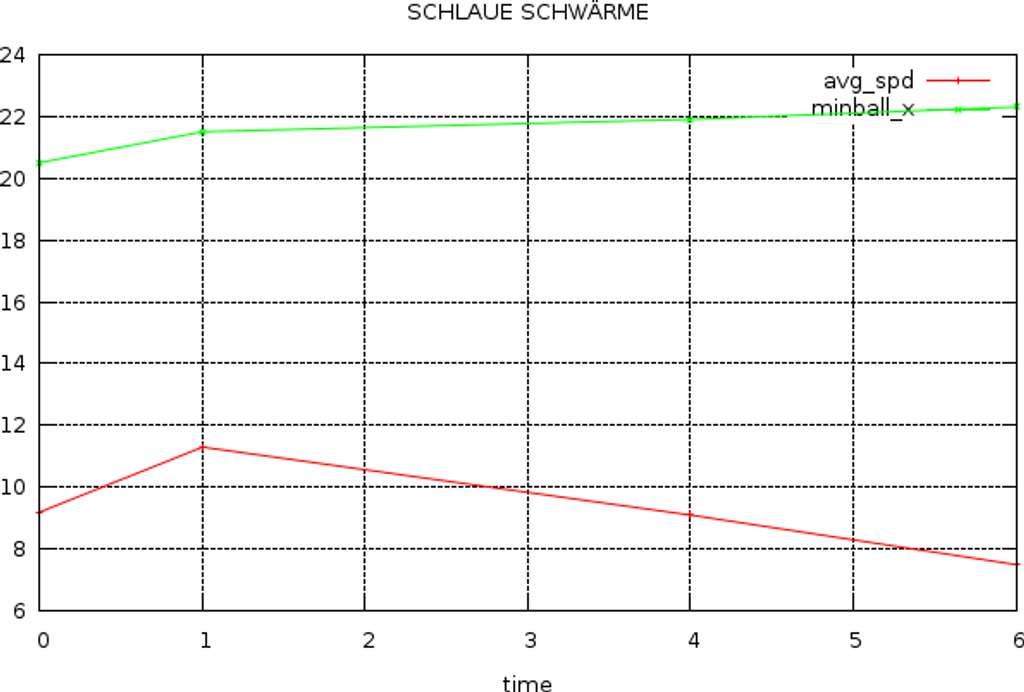
\includegraphics[width=0.9\textwidth]{stats-howto-gnuplot.png}
	\caption{Example result output from \gnuplot}
\end{figure}


\paragraph{More about \gnuplot}~\\

\begin{tabular}{l}
 $[1]$ Homepage: \texttt{\scriptsize http://www.gnuplot.info/} \\
 $[2]$ Introduction course: \texttt{\scriptsize http://userpage.fu-berlin.de/\~voelker/gnuplotkurs/gnuplotkurs.html}
\end{tabular}